
\providecommand{\myrootdir}{..}
\documentclass[\myrootdir/main.tex]{subfiles}

\begin{document}

\chapter{Chunk Retrieval Techniques for Build Logs}
\label{sec:techniques}
This chapter presents how a build log is created by a continuous integration (CI) build.
It explains our notion of retrievable information contained in build logs.
We introduce our notion of chunk retrieval techniques to retrieve information from build logs and present the three chunk retrieval techniques we investigate for this thesis:
Program synthesis by example (PBE), common text similarity (CTS) and keyword search (KWS).

\begin{figure}[htbp]
	\centering
	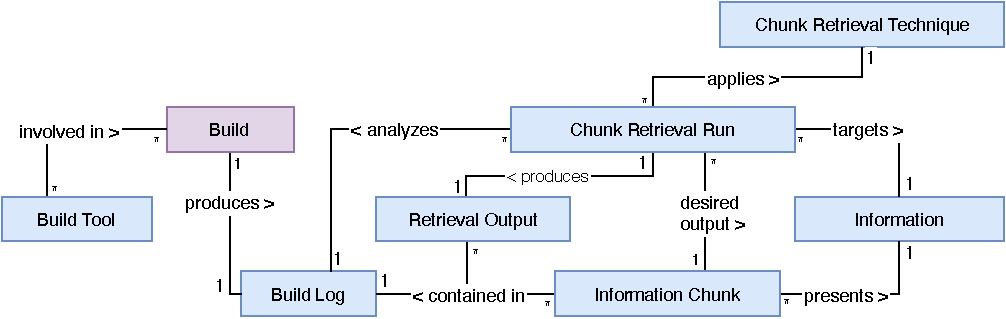
\includegraphics[width=\textwidth, clip]{img/build-overview.pdf}
	\caption{The different entities related to a CI build}
	\label{fig:build-overview}
\end{figure}

\section{Characteristics of a Build Log}
\label{sec:bl-characteristics}
The idea of CI is to catch errors early, by integrating new software changes fast and often~\cite{humble2010continuous}.
Companies often link a specific CI server, e.g.\ Travis CI, to their source code repository.
After making a change, the developer commits and pushes the new version of the code to the repository.
A push on specific branches or the creation of a pull request triggers a CI build.

A CI build typically runs through these stages:
\begin{itemize}
	\item Pulling the new, changed version of the source code into the build environment.
	\item Building the software, i.e.\ compiling and packaging it~\cite{phillips2014understanding}.
	\item Running static analysis tools~\cite{zampetti2017open}.
	\item Running automated tests~\cite{beller2017oops}.
	\item Deployment of the build artifact~\cite{schermann2016empirical}.
\end{itemize}

However, these are only \emph{typical} stages and there is a high variability in the CI build processes of different software projects~\cite{staahl2014modeling}.
Some smaller projects might use CI to just ensure their code compiles as a minimal check before reviewing a pull request.
Other projects might have various stages of extensive automated testing.

Software tools involved in the build write out log messages to the console.
They communicate progress updates, error and warning messages to the user~\cite{yuan2012characterizing}.
We refer to to the concatenation of this output as build log.
The structure of their output is chosen by every tool themselves.
Many have implicit or explicit structuring rules, some adhere to predefined standards like RSpec or PHPUnit~\cite{phpunit2019logging,rspec2019format}.
Figure~\ref{fig:tool-log-contribution} shows how different tools contribute to the whole build log.

\begin{figure}[htbp]
	\centering
	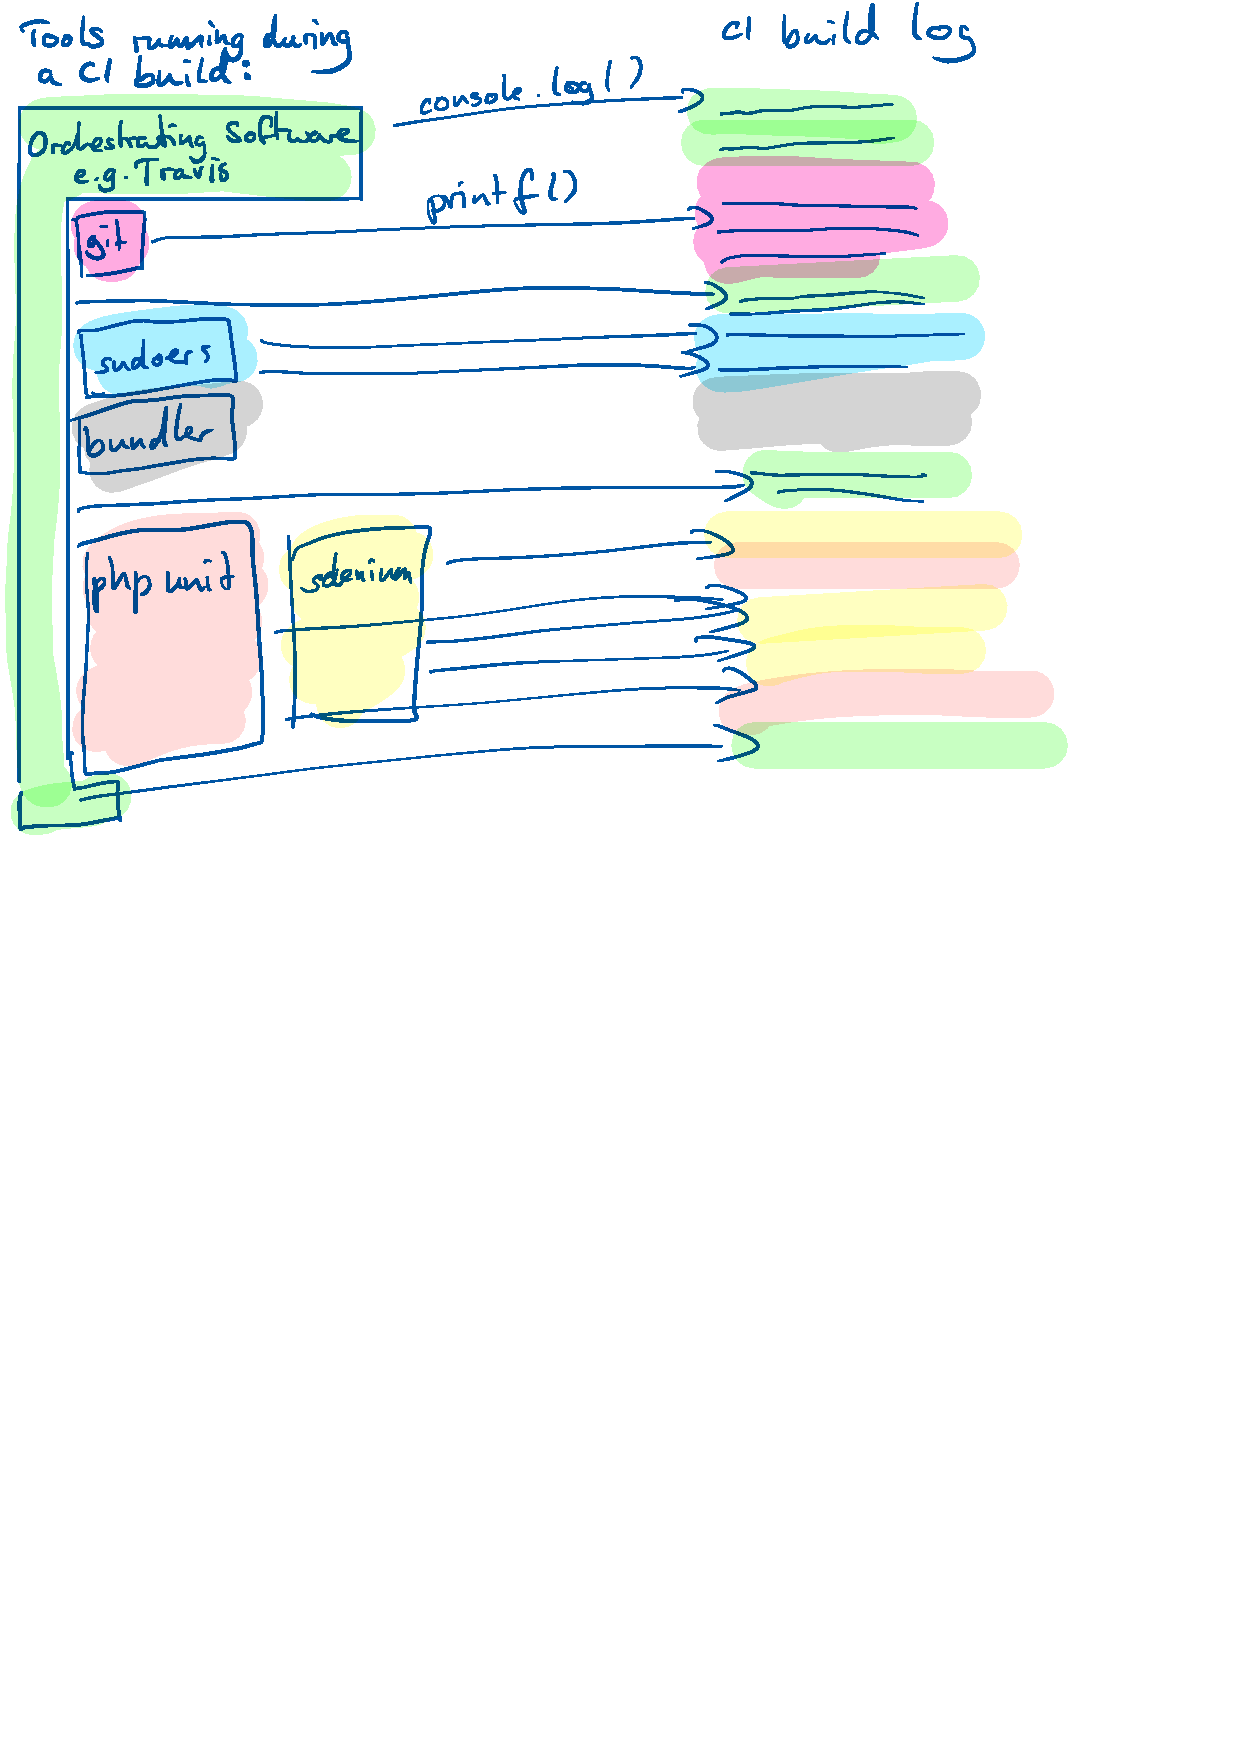
\includegraphics[width=\textwidth, trim={0cm 15cm 0cm 0cm}, clip]{img/tool-log-contribution.pdf}
	\caption{Contribution of different tools to the build log}
	\label{fig:tool-log-contribution}
\end{figure}

When analyzing build logs we might not have access to the exact build configuration, describing which tools are used in which order, or might not have access to a useable definition of the output structure of a specific tool.
Therefore build logs are semi-structured, as described in Section~\ref{sec:rw-semi-structured-data}.


\begin{figure}[htbp]
	\centering
	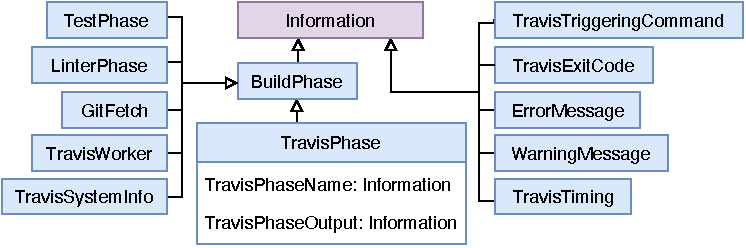
\includegraphics[width=\textwidth, clip]{img/build-log-information.pdf}
	\caption{Information retrievable from build logs}
	\label{fig:build-log-information}
\end{figure}

\section{Information Chunks in Build Logs}
\label{sec:bli}
CI build logs contain a great amount of information about the CI build they correspond to.
In this section we describe our notion of a information retrievable from a CI build log.
We present examples of information contained in Travis CI build logs and illustrate use cases for a developer or researcher to retrieve them.

The central class of our model is the \emph{BuildLogInformation} (BLI), representing a piece of information possibly retrievable from a build log.
\emph{Possibly}, because a BLI is not necessarily present in every build log.
If it is present, we call it a \emph{BuildLogInformation instantiation} (BLII), which always relates to a specific build log, the one this instantiation is appearing in.
Figure~\ref{fig:build-overview} presents the relation between a BLI and other entities involved in a CI build.

Each BLII for us has a \emph{textual representation} within the build log.
This textual representation is always a substring of the log text.
BLIs can be hierarchically ordered by their textual representations containing each other.
As this is an ad-hoc and a-posteriori structuring schema, as we describe in Section~\ref{sec:rw-semi-structured-data}, this section only presents hierarchical ordering or containment for BLIs whose structure we definitely know.
Most BLI types can appear in various hierarchical arrangements and are therefore not contained in any other type in our explanation.

During our initial exploration and log data collection for the \emph{Failing Build Log Data Set}, we collected a broad set of build logs from 29 languages and 87 repositories from Travis CI~\cite{travisci2019webpage}.
We inspected them to get an impression about the information one would want to retrieve from a build log.
In the following we describe the possibly interesting information types to be retrieved from Travis CI build logs.
All BLIs containing ``Travis'' in their name are specific to Travis CI build logs, the others can also apply to build logs from another CI environment.
Figure~\ref{fig:build-log-information} shows an overview of these BLIs.

\begin{itemize}
	\item \textbf{BuildPhase} Build logs can be divided into the sections produced by different tools.
	      These build steps could be for example be a \texttt{TestPhase}, \textbf{LinterPhase}, \textbf{TravisWorker}, \textbf{GitFetch}, or \textbf{Sudoers} are some that we encountered in the logs.

	\item \textbf{TravisPhase} Travis CI build logs consist of several build phases defined within the Travis CI configuration language. Within the build log each of these phases is framed by \lstinline{travis_fold:start:<travis phase name>} and \\ \lstinline{travis_fold:end:<travis phase name>}.

	      A TravisPhase always contains:
	      \begin{itemize}
		      \item \textbf{TravisPhaseName} The string Travis CI uses to identify the phase within start and end statements.
		      \item \textbf{TravisPhaseOutput} The output generated during the travis phase. The textual representation of the \texttt{TravisPhaseOutput} instantiation is the substring between the start and end statements.
	      \end{itemize}
				 Retrieving the names of the phases of a Travis CI build log could be used to afterwards reconstruct an overview of the executed steps within a build.
	       Figure~\ref{fig:log-1} shows an example of a TravisPhase instantiation and its components within a build log.

	\item \textbf{TravisTiming} Travis can measure the time of specified sections of the build process.
				A developer can retrieve this timing information to automatically monitor the performance of their build.
	      Figure~\ref{fig:log-1} shows an example of a TravisTiming instantiation.
	      %It represents those by \lstinline{travis_time:start:<timing section id>} and \\ \lstinline{travis_time:end:<timing section id>:start=<start time>,finish=<finish time>,duration=<duration>}

	\item \textbf{TravisWorker} Travis CI mentions for each build which machine is executing the build.
	      Retrieving this information from multiple build logs can help visualize the impact of the build server assignment algorithm.
	      The TravisWorker is a good example that the same BLI can have different textual representations in different build logs.
	      Figure~\ref{fig:log-0} and Figure~\ref{fig:log-2} show examples of different TravisWorker instantiations.

	\item \textbf{TravisSystemInfo} At the beginning of each log Travis CI describes the tech stack of the server executing the build.
				A developer can retrieve the system information from both failing and successful logs to identify if a failure could be based on the execution environment.
	      Figure~\ref{fig:log-0} shows an example of a TravisSystemInfo instantiation within a build log.

	\item \textbf{TravisTriggeringCommand} Travis CI logs the commands it uses to call certain tools.
	      These come from the \texttt{travis.yml} configuring the build.
				This information can be useful for a researcher to retrieve when reverse engineering the build configuration.
	      Figure~\ref{fig:log-3} shows an example of a TravisTriggeringCommand instantiation.

	\item \textbf{ExitCode} Travis CI prints all exit codes of commands.
				A researcher can retrieve this information to fill an overview of the build steps and why they failed.
	      Figure~\ref{fig:log-3} shows an example of an ExitCode instantiation within a build log.

	\item \textbf{ErrorMessage} Various tools involved in the build process output messages of errors that occurred during their execution.
	      Retrieving these and showing them to developers can help them understand quicker why the build failed.
	      Figure~\ref{fig:log-3} shows an example of and ErrorMessage instantiation.

	\item \textbf{WarningMessage} In addition to errors, tools also print warning messages.
				Developers can collect and count them to encourage their team to resolve them.
	      Figure~\ref{fig:log-4} and Figure~\ref{fig:log-5} show examples of WarningMessage instantiations within build logs.

\end{itemize}

\begin{figure}[htbp]
	\centering
	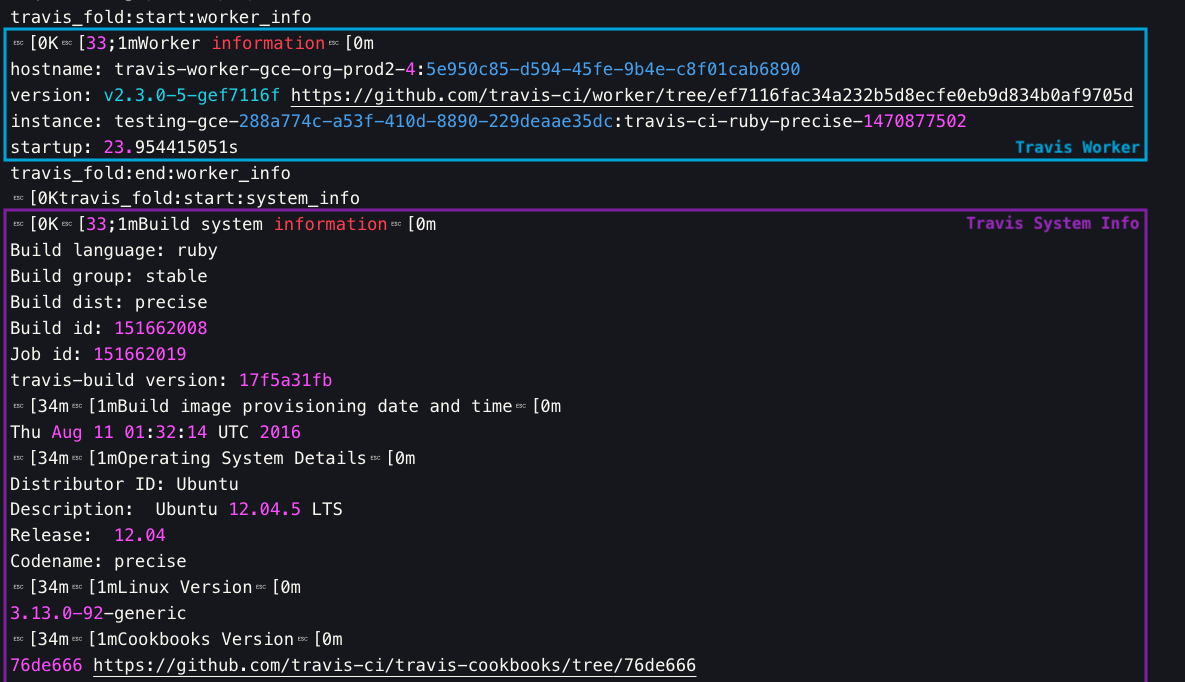
\includegraphics[width=\textwidth, clip]{img/log0.png}
	\caption{Excerpt from a build log showing textual representations of a long TravisWorker instantiation and a TravisSystemInfo instantiation}
	\label{fig:log-0}
\end{figure}
\begin{figure}[htbp]
	\centering
	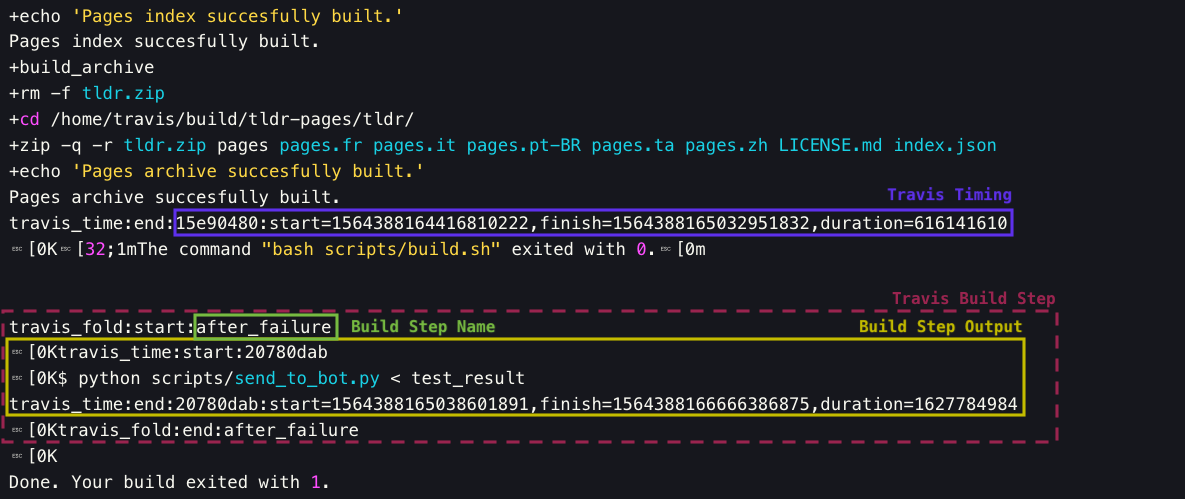
\includegraphics[width=\textwidth, clip]{img/log1.png}
	\caption{Excerpt from a build log showing textual representations of a TravisTiming instantiation and a TravisPhase, containing the TravisPhaseName and the TravisPhaseOutput}
	\label{fig:log-1}
\end{figure}
\begin{figure}[htbp]
	\centering
	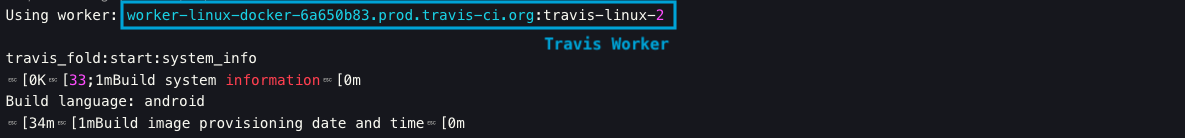
\includegraphics[width=\textwidth, clip]{img/log2.png}
	\caption{Excerpt from a build log showing textual representations of a short TravisWorker instantiation}
	\label{fig:log-2}
\end{figure}
\begin{figure}[htbp]
	\centering
	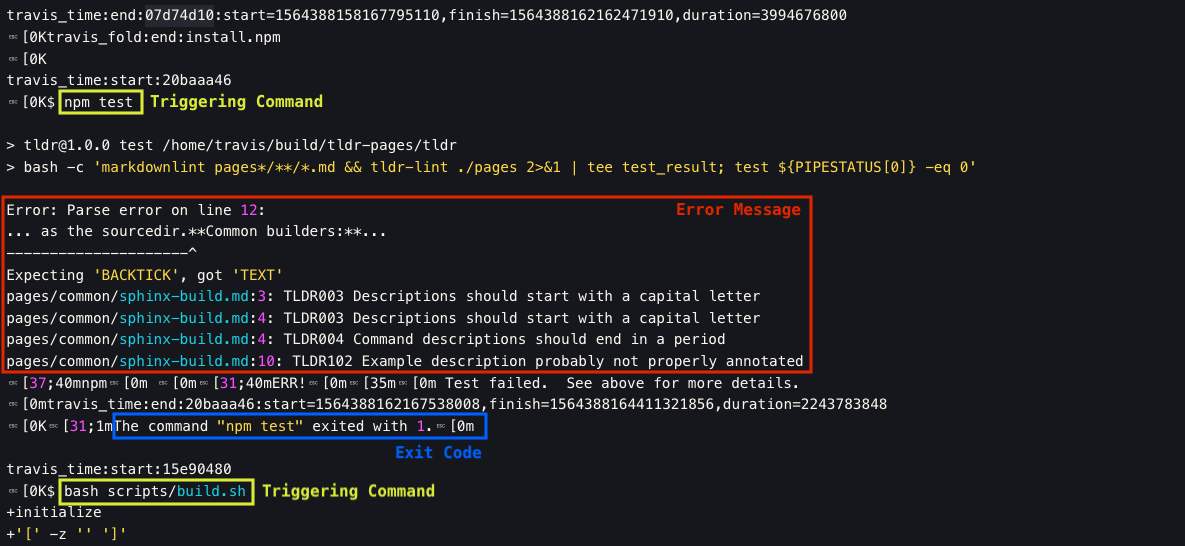
\includegraphics[width=\textwidth, clip]{img/log3.png}
	\caption{Excerpt from a build log showing textual representations of ErrorMessage, ExitCode and TravisTriggeringCommand instantiations}
	\label{fig:log-3}
\end{figure}
\begin{figure}[htbp]
	\centering
	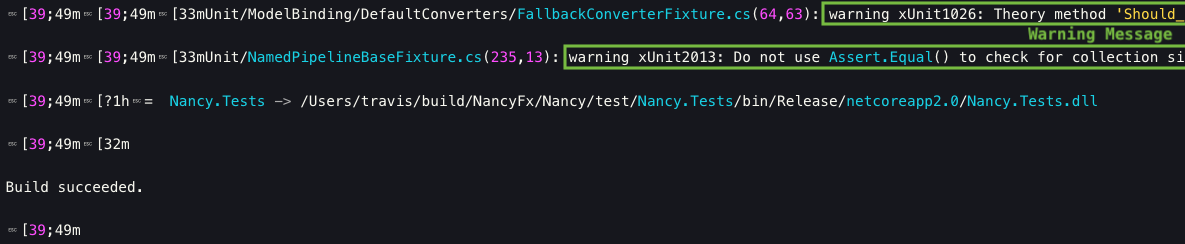
\includegraphics[width=\textwidth, clip]{img/log4.png}
	\caption{Excerpt from a build log showing textual representations of WarningMessage instantiations}
	\label{fig:log-4}
\end{figure}
\begin{figure}[htbp]
	\centering
	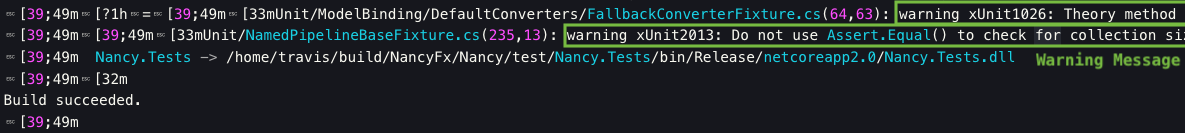
\includegraphics[width=\textwidth, clip]{img/log5.png}
	\caption{Excerpt from a build log showing textual representations of WarningMessage instantiations}
	\label{fig:log-5}
\end{figure}


\begin{figure}[htbp]
	\centering
	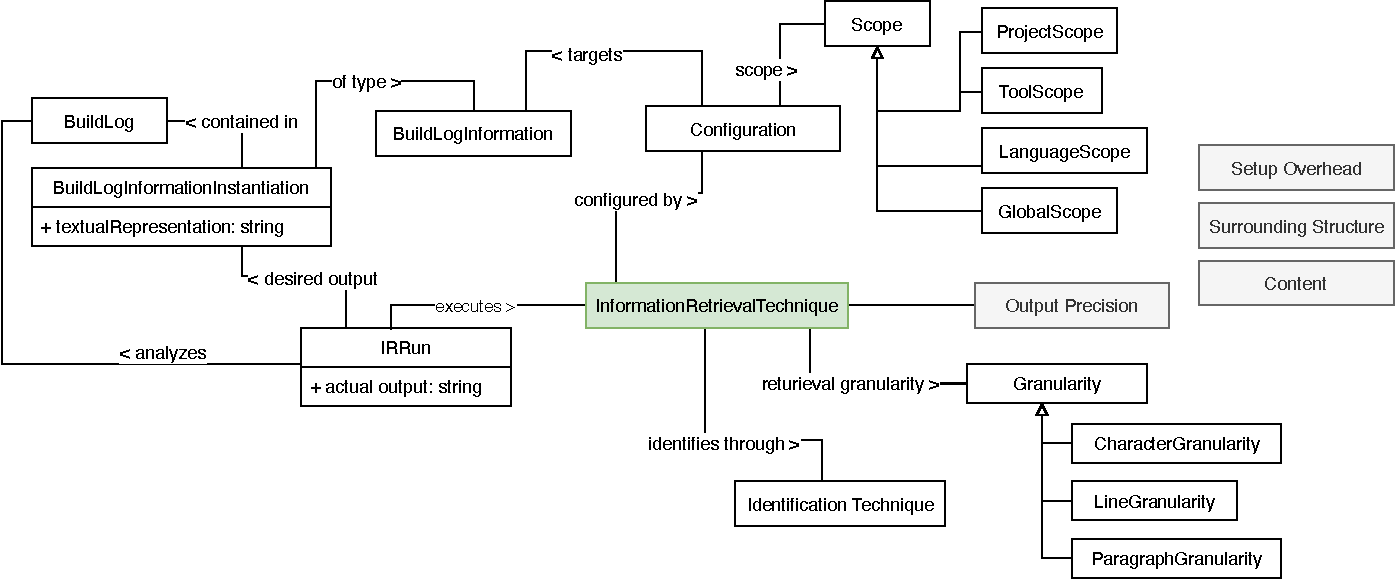
\includegraphics[width=\textwidth, clip]{img/ir-technique.pdf}
	\caption{Model for an Information Retrieval Technique}
	\label{fig:model-ie-technique}
\end{figure}
\section{Characteristics of Chunk Retrieval Techniques}
\label{sec:blirt}
For this thesis, we want to evaluate different \emph{chunk retrieval techniques} (CRTs) when applied to CI build logs.
A chunk retrieval does not require to parse the structure of a whole build log.
It focus on extracting just one information, specified by its configuration.

Each CRT has a specific \textit{granularity}, i.e.\ the smallest retrievable text piece and uses a specific \textit{identification technique} to select the log parts it retrieves.
The \textit{configuration} instantiates a CRT to target a specific BLI and supplies the necessary information for the CRT to identify the textual representation of the targeted BLI in a build log.
Each configuration addresses a specific \textit{scope}.
The scope an be a specific project, a tool involved in the build, a programming language or global, configuring a retrieval technique for all possible build logs.
A \textit{CRT run} consumes a build log as a plain text file and produces a string output, which consists of substrings of the build log text.

The following sections of this chapter introduce the three CTRs we investigate: Program synthesis by example (PBE), common text similarity (CTS) and keyword search (KWS).
Lastly we describe other techniques which can also be comprehended as CRTs.
Table \ref{tab:ctr} shows a comparison of the presented techniques.

\begin{table}[htbp]
\centering
\caption{Chunk Retrieval Techniques}
\begin{tabularx}{\textwidth}{|X|l|X|l|X|} 
\hline
Name                         & Acronym & Identification Technique                                   & Granularity & Configuration             \\ 
\hline
\hline
Program Synthesis by Example & PBE     & Regular expression program                                 & Character   & In / Output Examples      \\
\hline
Common Text Similarity       & CTS     & Tf-idf \& cosine similarity, mean number of lines expected & Line        & Output Examples           \\
\hline
Keyword Search               & KWS     & Keywords, mean number of lines expected                    & Line        & Keywords, Context Length  \\
\hline
Random Line Retrieval        & RLR     & Random sample                                              & Line        & Retrieval Length          \\
\hline
Diff Approach                &         & Line not present in successful log                         & Line        & Successful Log File       \\
\hline
\end{tabularx}
\label{tab:ctr}
\end{table}

\subsection{Program Synthesis by Example (PBE)}
\label{sec:expl-pbe}
\emph{Programming by Example} is a technique which synthesizes programs according to in and output examples provided by the user.
It enables users to create programs without a priori programming knowledge~\cite{mayer2015user}.
In the context of text extraction through regular expressions, Programming by Example relieves the developer from having to understand the whole document structure to solve a single extraction task~\cite{le2014flashextract:}.
We chose to investigate the applicability of generating regular expression programs by example to retrieving information chunks from build logs.
In this work, we refer to our interpretation of Programming by Example as \emph{PBE}.
In the following we will explain the concept of how we apply PBE to chunk retrieval from CI build logs, the concrete implementation is described in~\ref{sec:impl-pbe}.
%Figure~\ref{fig:prose-explanation} shows the instantiation of the BLIRT model for PBE\@.

\paragraph{Configuration}
In/output examples (I/O examples) are the main driver of Programming by Example.
When retrieving information chunks from build logs the \emph{input} is always a whole build log, i.e.\ the whole text of the build log file.
The \emph{output} is always a substring of the log file text, representing the substring that should be retrieved by the synthesized program when given the corresponding input file.
One or multiple I/O examples configure a chunk retrieval with PBE, they define the substring of a build log that should be extracted.
The PROSE program synthesis then tries to construct a regular expression program consistent with all configuring I/O examples.
A program is consistent with an I/O example if it returns the defined output when executed on the defined input.
PBE reports an error back to the user if no consistent program could be synthesized.
The program synthesis builds on the Flash Extract DSL, which in turn uses the FlashMeta algorithm.
Both are described in Section~\ref{sec:rw-prose}.

\paragraph{Application}
A CTR run with PBE takes a build log file as input and applies the synthesized regular expression program.
It then returns the substring of the build log matched by the program or an empty string if the program found no match.
%For execution PBE takes a build file as input and returns a substring of the build file content.

\subsection{Common Text Similarity (CTS)}
\label{sec:expl-ts}
Text Similarity approaches are more and more used to filter unstructured textual software artifacts~\cite{runeson2007detection,marcus2005recovery,antoniol2002recovering,mccarey2006recommending}.
One common and simple technique the Vector Space Model~\cite{schutze2008introduction}.
We investigate when text similarity is a suitable technique to retrieve information chunks from build logs.
In the following we will explain the concept of how we apply text similarity to information retrieval from CI build logs (CTS), the concrete implementation is described in~\ref{sec:impl-ts}.
%Figure~\ref{fig:text-similarity-explanation} shows the instantiation of the BLIRT model for CTS.

\paragraph{Configuration}
To configure a chunk retrieval though text similarity we chose to use the same concept of I/O examples as for PBE\@.
The lines of the output strings of the configuring I/O examples define our search query.
The algorithm splits the search query into single lines and identifies tokens, in our case words.
%Commonly text similarity techniques employ further normalization like removing special characters and stop words.
%We chose to keep the build log lines as complete as possible, as we often saw special characters and words identifying an interesting area.
Then we build a document-term-frequency matrix over the lines from the search query and prune very often or very rarely appearing words.
Next, the algorithm applies term-frequency inverse document frequency to the matrix, a best practice for natural language queries~\cite{lee1997document}.

\paragraph{Application}
To retrieve the desired information from a build log, we parse the whole text and process it in the same way as the search query.
The algorithm calculates the cosine similarity~\cite{korenius2007principal} to compare each line of the build log with each line of the search query.
After summing up the similarities of each build log line to all search query lines, we sort the build log lines in decreasing similarity.
The average number of lines in the outputs of the configuring I/O examples determines how many of the most similar lines are returned as the output of the retrieval run.

\subsection{Keyword Search (KWS)}
\label{sec:expl-skws}
When developers are looking for a specific piece of information within a great amount of unstructured information, they search for related keywords as a first ad-hoc approach.
This was one of the most common approaches we took when searching for the build failure reason within a log when creating our \emph{Failing Build Logs Data Set}.
As this is a technique readily available in many tools developers use to view build logs, we want to study when such a keyword search is recommendable for retrieving information chunks from CI build logs.
In the following we will explain how we use simple keyword search to retrieve information from CI build logs (KWS), the concrete implementation is described in~\ref{sec:impl-skws}.
%Figure~\ref{fig:keyword-search-explanation} shows the instantiation of the BLIRT model for SKWS.

\paragraph{Configuration}
A set of keywords configures the chunk retrieval with KWS.
To better compare KWS with PBE and CTS, we also configure it through I/O examples.
We link each I/O example with keywords, which appear in the desired output or close to it in the input build log.
The configuring keywords for KWS are the ones that appear most often in the keywords of the configuring I/O examples.

\paragraph{Application}
For a retrieval run, we take a whole build log file as input and search for all exact occurrences of the configuring keywords.
As keywords are often not directly describing the desired information but rather adjacent to the desired information, this technique retrieves the lines around not only retrieves the line with the keyword but also the lines around it.
The number of surrounding lines retrieved is the average of lines in the output of the configuring I/O examples.

\subsection{Other Techniques}
\label{sec:expl-rlr}
Apart from the three techniques we investigate, there are further build log analysis techniques mentioned in literature and used in industry.
This section shows how they are described with our notion of chunk retrieval techniques.

\paragraph{Log Diff}
Amar et al.\ use a technique based on line diffs to retrieve relevant lines from a failed build log~\cite{amar2019mining}, as we describe in more detail in Section~\ref{sec:rw-bl-analysis}.
The configuration for the technique is the log from the last successful build.
This techniques retrieves all lines from a build log which are not present in the configuring build log.
%Figure~\ref{fig:diff-technique-model} shows how this technique would be in our BLIRT model.
\paragraph{Random Line Retrieval (RLR)}
In our evaluation we want to compare against a baseline of randomly extracted lines.
The average number of lines in the outputs of a set of I/O examples is the configuration for random line retrieval (RLR).
It retrieves this number of lines randomly sampled from the build log.

\end{document}
